\documentclass[a4paper, 12pt]{article}
\usepackage{tikz}
\usepackage[top=0.5in]{geometry}
\usetikzlibrary{automata, positioning}
\usepackage{comment}
\begin{document}

\noindent\large\textbf{Problem 1a}
\\
\\
NFA N$\colon$
\\
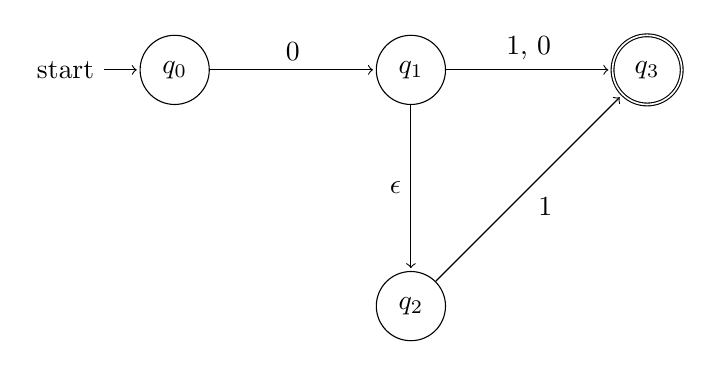
\begin{tikzpicture}[shorten >=1pt, node distance=3cm, on grid, auto]
    \node[state,initial] (q_0)	{$q_0$};
    \node[state] (q_1) [right=of q_0] {$q_1$};
    \node[state] (q_2) [below=of q_1] {$q_2$};
    \node[state, accepting] (q_3) [right=of q_1] {$q_3$};
	\path[->]
	(q_0) edge node {0} (q_1)
	(q_1) edge node {1, 0} (q_3)
	(q_1) edge node [swap] {$\epsilon$} (q_2)
	(q_2) edge node [swap] {1} (q_3);
\end{tikzpicture}
\\
The language of NFA N accepts the strings $\{01, 00\}$. After flipping the states we get the NFA M$\colon$
\\
\\
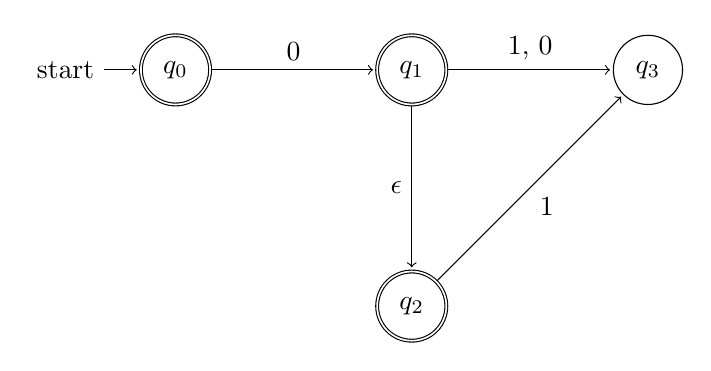
\begin{tikzpicture}[shorten >=1pt, node distance=3cm, on grid, auto]
    \node[state,initial, accepting] (q_0)	{$q_0$};
    \node[state, accepting] (q_1) [right=of q_0] {$q_1$};
    \node[state, accepting] (q_2) [below=of q_1] {$q_2$};
    \node[state] (q_3) [right=of q_1] {$q_3$};
	\path[->]
	(q_0) edge node {0} (q_1)
	(q_1) edge node {1, 0} (q_3)
	(q_1) edge node [swap] {$\epsilon$} (q_2)
	(q_2) edge node [swap] {1} (q_3);
\end{tikzpicture}
\\
Which accepts the strings $\{\epsilon, 0\}$ which is not the complement of N.
\\
\\
\noindent\large\textbf{Problem 1b}
\\
\\
DFA's are closed under complement and NFA's and DFA's recognize the same class of languages.  Therefore the class of languages recognized by an NFA are closed under complement.
\\
\\
\noindent\large\textbf{Problem 2}
\\
\\
A and B are regular languages. The complement of A and the complement of B both are closed under complement and thus will produce a language that is regular.  The complement of that language, C, is also regular. 
\[\overline{\overline{\textbf{A}} \cup \overline{\textbf{B}}} = \textbf{C}\]
By DeMorgan's Law, we have the intersection of A and B. Thus, The class of regular languages are closed under intersection. 
\[\textbf{C} = \textbf{A} \cap \textbf{B}\]
\\
\\
\noindent\large\textbf{Problem 3}
\\
\\
A DFA M = $\left(Q, \sigma, \delta, q_{0}, F\right)$, recognizes a regular language A. We will construct an NFA N by switching the direction of the transition arrows, swapping the start and acceptance states, and adding $\epsilon$ transitions. We then have the NFA N = $\left( Q\prime, \sigma\prime, \delta\prime, q_{0}\prime, F\prime \right)$ which recognizes $A^{R}$.
\end{document}
